\documentclass[UTF8]{ctexart}

\usepackage{subfiles}  

%下面的语句, 引入你的头部设置文件
\usepackage{C:/phpStorm_proj/02_myself_ID_EGO/+100_latex_all_math_sel/myPreamble} 
%必须是绝对路径,才能让各个tex在单独编译时使用到

\title{文件名}


%---------------------------------


\begin{document}
	\tableofcontents % 生成目录
	\date{} % 若不写这句, 则默认也会渲染出日期, 所以我们要手动赋空值
	\maketitle  %这行代码, 让你前面的 title, author, date生效
	
	
	
	\part{条件概率}
	
	\section{``条件概率"的意思}
	
	条件概率是: 有A, B 两个事件, 和样本空间 Ω. 其中 $P(B) >0$, 则, 在B已经发生的条件下, A发生的概率, 就叫做A对B 的``条件概率". 记作:  P(A| 条件B), 读作``在B发生的条件下, A发生的概率”. \\
	
	即, 条件概率公式是: $
	\text{P}\left( \text{A|\ 条件B} \right) =\dfrac{\overset{\text{这个分子即:\ AB同时发生了}}{\overbrace{\text{在B发生条件下,A发生的样本点数}}}}{\text{B里面有多少个样本点}}=\dfrac{\text{n}_{\text{AB}}}{\text{n}_{\text{B}}}
	$ \\
	
	还可写成:  $
	\text{P}\left( \text{A|\ 条件B} \right) 
	=\dfrac{\text{P}\left( \text{A}\cap \text{B} \right)}{\text{P}\left( \text{B} \right)}
	=\dfrac{\frac{\text{n}_{\text{AB}}}{\text{n}}}{\dfrac{\text{n}_{\text{B}}}{\text{n}}}=\dfrac{\text{n}_{\text{AB}}}{\text{n}_{\text{B}}}
		$ \\
	
	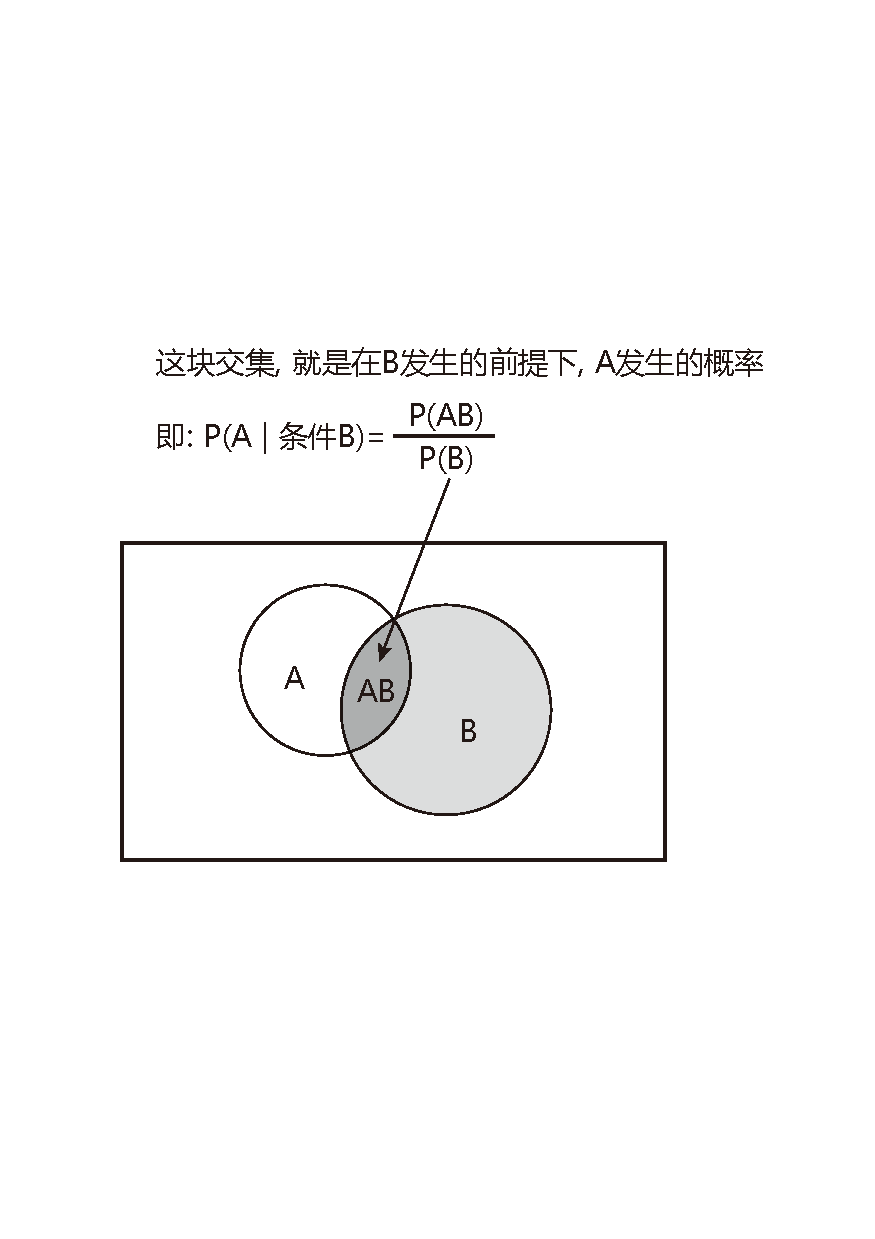
\includegraphics[width=0.5\textwidth]{/0088.pdf} \\
	
	如上图所示, 注意: 概率是个比值, 所以你光有分子那块的交集值, 是没用的, 它还需要与另一个数(分母)去比. \\
	
	上面公式中, P(AB) 的计算公式是什么呢? \\
	- 如果事件A, 和事件B 是相互独立的, 则 $P(AB) = P(A) \cdot P(B)$ \\
	- 如果事件A, 和事件B 不相互独立, 则只能用``条件概率"公式, 来求P(AB), 即: $P(AB) = P(A |B) \cdot P(B) = P(B |A) \cdot P(A) $   \\
	
	
	
	注意: ``条件概率", 和``分步骤法"的区别: \\
	- 分步骤法: 前后每一步骤的事件是相互独立的, 彼此没有条件关系.  \\
	比如, 第一步你结婚, 第二步我结婚. 我们这两件事发生的概率互不影响. \\
	
	- 条件概率: 前面的事件, 有可能会(但并不一定)影响到后面事件的发生概率. 即前后事件之间并不互相独立.  \\
	会影响的例子: 比如一共有100个上岸机会, 则第一步你上岸的成功概率, 会影响到第二步我上岸的成功概率. (你若成功, 留给我的名额数量就会更少.) \\
	彼此独立的例子: 比如在你回国的条件下, 我出门的概率. 两者发生的概率毫无关系. 你回不回国, 跟我会出不出门没半毛钱关系.
	
	
	
	
	
	
	
	
	
	
	\begin{myEnvSample}
		有6个球, 各有编号.  我们先定义下这些事件: \\
		- B: 取到偶数编号的球 \\
		- $A_1$: 取到1号球 \\
		- $A_2$: 取到2号球 \\
		- $A_5$: 取到大于4号的球 \\
		
		则: \\
		- $
		\overset{\text{取到1号球的概率}}{\overbrace{\text{P(A}_1\text{)}}}=\frac{\overset{1\text{号球选}1}{\overbrace{\text{C}_{1}^{1}}}}{\underset{\text{全6选}1}{\underbrace{\text{C}_{6}^{1}}}}=\frac{1}{6}=0.166667
		$
		
		- $
		\text{P}\left( \text{A}_1|\text{B} \right) =\frac{\text{在B条件里面,取到A}_1\text{(即1号球)}}{\text{B:\ 取到偶数编号的球}}=\frac{\overset{\text{偶数编号的球里面,\ 取不到奇数编号的球}}{\overbrace{0}}}{\underset{3\text{个偶数球里面取1个}}{\underbrace{\text{C}_{3}^{1}}}}=0
		$
		
		- $
		\text{P}\left( \text{A}_2|\text{B} \right) =\frac{\overset{1\text{个编号2的球里面,取1个}}{\overbrace{\text{C}_{1}^{1}}}}{\underset{3\text{个偶数球里面取1个}}{\underbrace{\text{C}_{6}^{3}}}}=\frac{1}{3}
		$
		
		- $
		\text{P}\left( \text{A}_5|\text{B} \right) =\frac{\text{在B条件里面,取到大于4号的球}}{\text{B:\ 取到偶数编号的球}}=\frac{\overset{5,6\text{号与偶数的交集,\ 只有6号一个球}}{\overbrace{1}}}{3}
		$
			
	\end{myEnvSample}
	
	
	~\\
	\hrule
	~\\
	
	
	\section{条件概率的性质}
	
	\subsection{性质: $ P(A | \text{条件}B) >= 0$}
	
	
	\subsection{性质: $ P(\Omega | \text{条件}B) = 1$}
	
	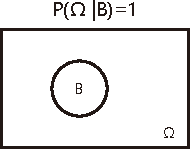
\includegraphics[width=0.25\textwidth]{/0089.pdf}
	
	
	\subsection{性质: $ \text{P}\left( \text{A}_1\cup \text{A}_2\ |\text{B} \right) =\text{P}\left( \text{A}_1\ |\text{B} \right) +\text{P}\left( \text{A}_2\ |\text{B} \right) -\text{P}\left( \text{A}_1\text{A}_2\ |\text{B} \right) 		$}
	
	\subsection{性质: $	\text{P}\left( \text{A\ |B} \right) =1-\text{P}\left( \overline{\text{A}}\ |\text{B} \right) 	$}
	
	\subsection{性质: 可列可加性:  若$ A_1, A_2, ... A_n, ...$ 是``互不相容"的事件, 则有: $ P(\sum_{i=1}^\infty A_i | B) = \sum_{i=1}^ \infty P(A_i | B)$ ← 即: ``和的概率", 等于``概率的和"}
	
	
	
	
	~\\
	\hrule
	~\\
	
	
	\section{``条件概率"的乘法公式 : $ P(\text{前后})=P(\text{后}) \cdot P(\text{前}|\text{\text{后}}) = P(\text{\text{前}}) \cdot P(\text{后}|\text{前})$}

	推导过程: \\
	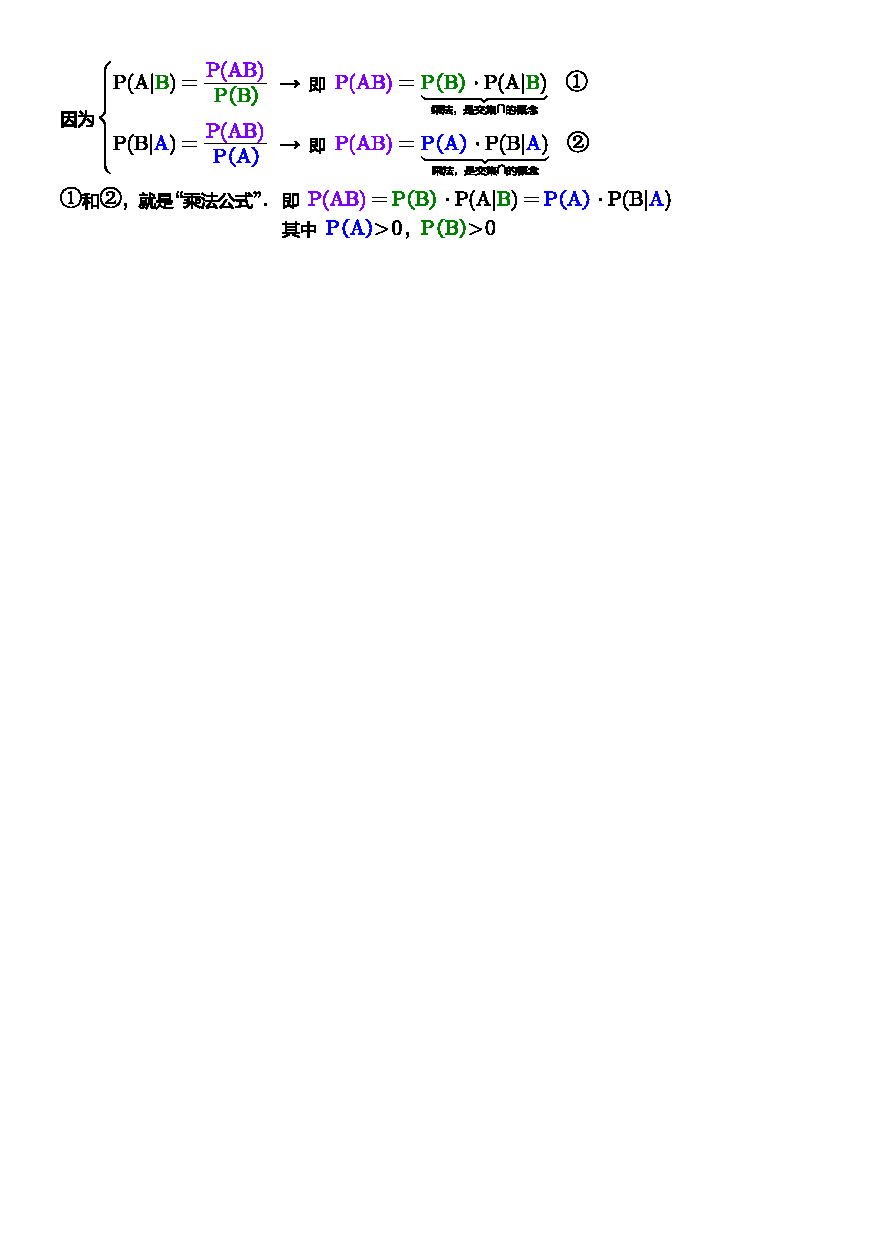
\includegraphics[width=0.8\textwidth]{/0090.pdf} \\
	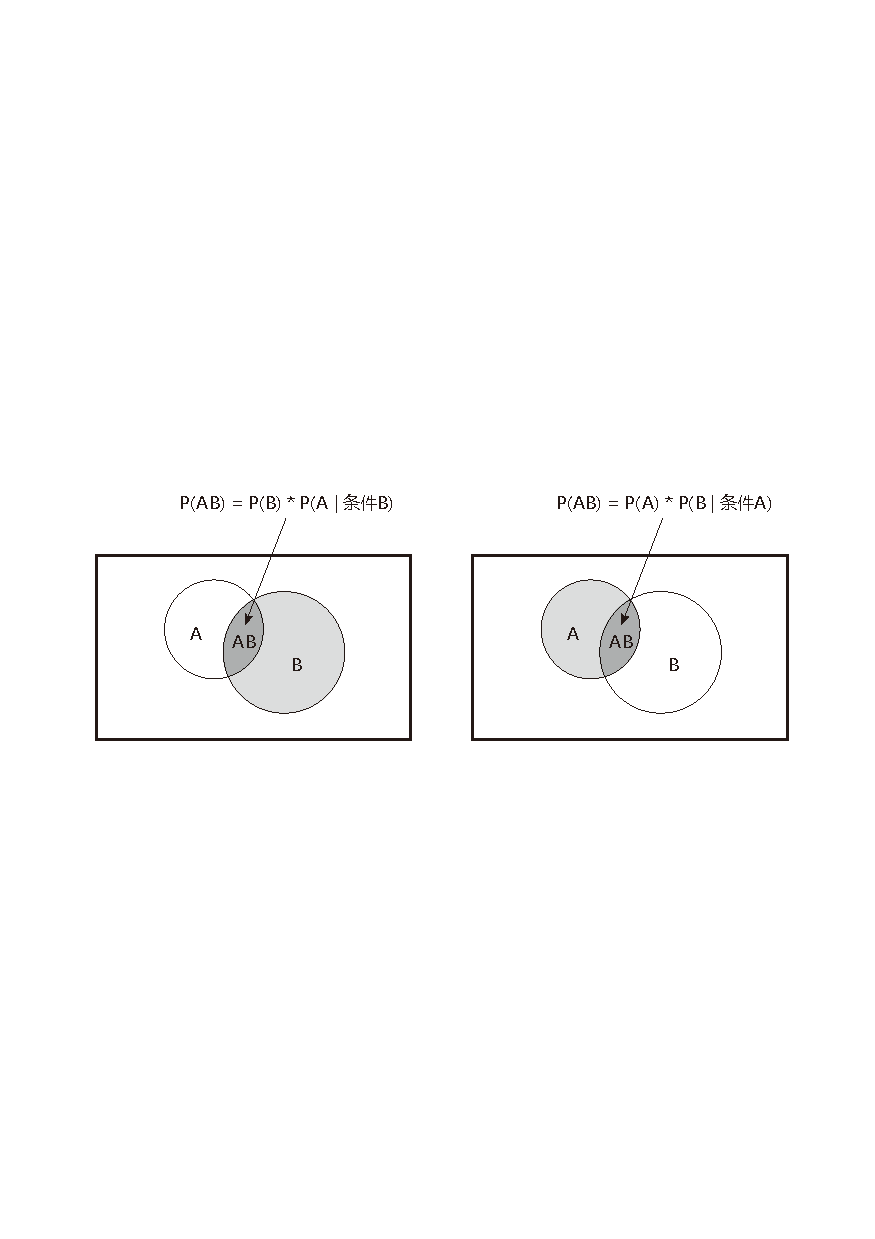
\includegraphics[width=0.8\textwidth]{/0091.pdf} \\
	
	同理, 多个事件的乘法公式就是:  \\
	→ $ \boxed{
	\text{P(ABC)}=\underbrace{\text{P(A)}}\cdot \underbrace{\text{P(B|A)}}\cdot \underbrace{\text{P(C|BA)}} 	
	}
	$ \\
	↑ 上面``从右往左"看, 就是按 A,B,C 的顺序 \\
	
	→ 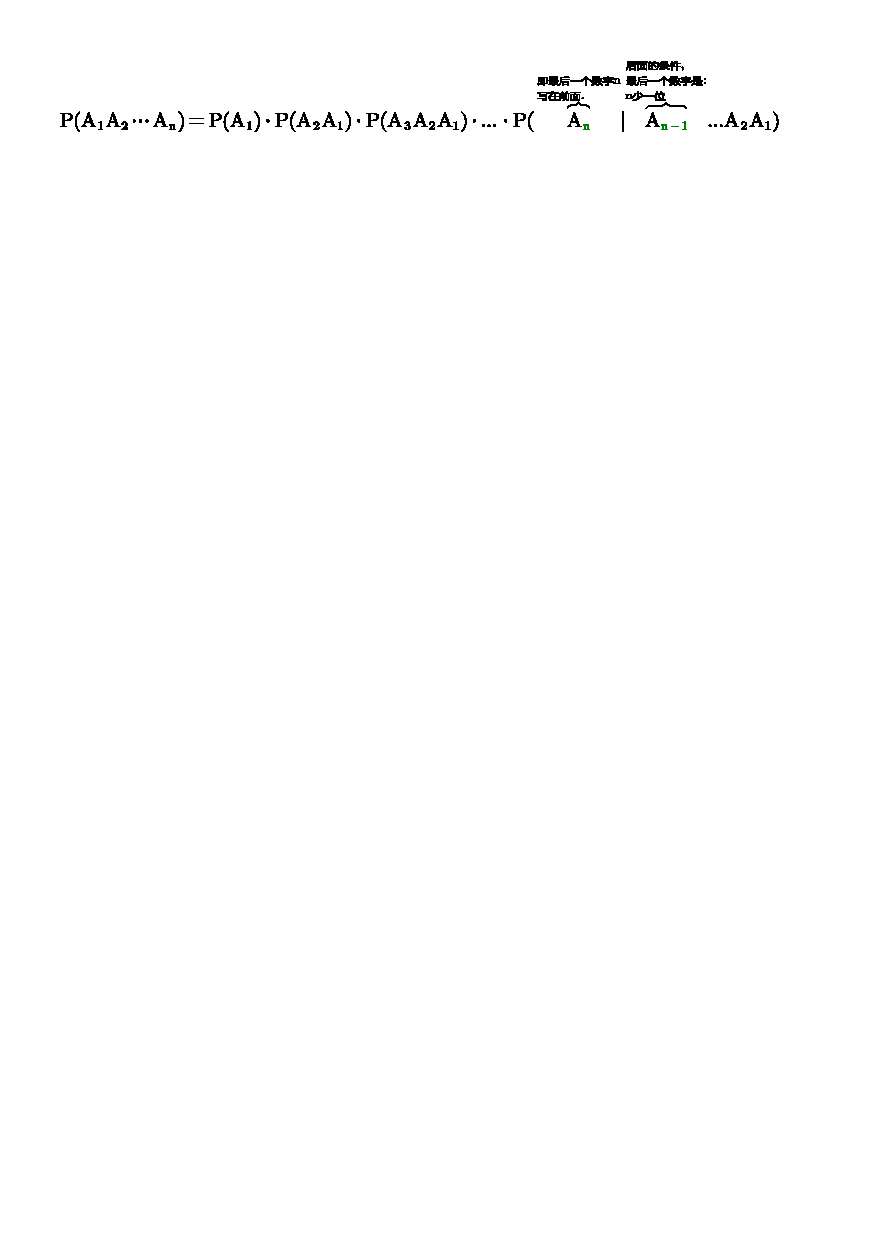
\includegraphics[width=0.95\textwidth]{/0092.pdf} \\
	↑ 上面``从右往左"看, 就是按$A_1, A_2, ... , A_n$的顺序 \\
	
	
	\begin{myEnvSample}
		有100件产品, 次品率=10\%, 即有10件次品. 做不放回抽样, 问: 第3次才取到合格品的概率是? \\
		我们先令: \\
		- $A_1$ 表示第1次取, 就取到了合格品 \\
		- $A_2$ 表示第2次取, 取到了合格品 \\
		- $A_3$ 表示第3次取, 取到了合格品 \\
		
		那么第3次才取到合格品, 就是:  \\
		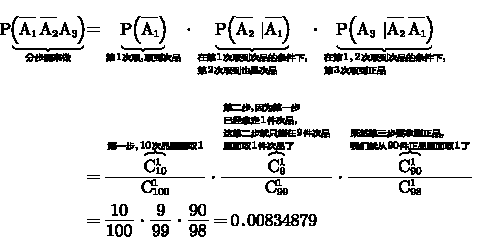
\includegraphics[width=0.8\textwidth]{/0093.pdf} 		
	\end{myEnvSample}
	
	


\begin{myEnvSample}
	某产品:  \\
	- 甲公司占60\%市场份额, 且其产品合格率是 90\% \\
	- 乙公司占40\%市场份额, 且其产品合格率是 80\% \\
	
	我们先定义下这些事件: \\
	- J: 表示产品是甲的 \\
	- $\overline{\text{J}}$: 表示产品是乙的 \\
	- Q (qualified) : 表示产品是``合格"的 \\
	- $\overline{\text{Q}}$ : 表示产品是``不合格"的 \\
	
    问, 你买一个产品, 是甲公司的, 并且是合格的概率是? \\
    $
    \text{P}\left( \text{JQ} \right) =\underset{=0.6}{\underbrace{\text{P}\left( \text{J} \right) }}\cdot \underset{\text{甲的合格率}=0.9}{\underbrace{\text{P}\left( Q \ | J \right) }}=0.54
    $ \\
    
    问, 你买一个产品, 是乙公司的, 并且是合格的概率是? \\
    $
    \text{P}\left( \overline{\text{J}}\text{Q} \right) =\underset{=0.4}{\underbrace{\text{P}\left( \overline{\text{J}} \right) }}\cdot \underset{\text{乙条件下的合格率}=0.8}{\underbrace{\text{P}\left(Q \ | \overline{\text{J}} \right) }}=0.32
    $      
\end{myEnvSample}





\begin{myEnvSample}
	抽签, 共10签, 其中有4个为``成功上岸"的好签. 甲乙丙三人, 按顺序依次去抽, 不放回. \\
	我们先设定事件:  \\
	- A: 表示甲 抽到``成功" \\
	- B: 表示乙 抽到``成功" \\
	- C: 表示丙 抽到``成功" \\
	
	问, (1) 甲抽到``成功"的概率? 
	$
	\text{P}\left( \text{A} \right) =\dfrac{\text{C}_{4\text{好签}}^{1}}{\text{C}_{10\text{签}}^{1}}=\frac{4}{10}=0.4
	$ \\
	
	(2) 甲乙都抽到``成功"的概率?  
\begin{align*}  % 支持每行编号. 若不需要编号, 就用 align*环境
	&\text{P}\left( \text{AB} \right) =\underset{\text{第1步:甲先成功}}{\underbrace{\text{P}\left( \text{A} \right) }}\cdot \underset{\text{第2步:在甲成功的前提下,\ 乙再成功}}{\underbrace{\text{P}\left( \text{B\ |A} \right) }}\\
&=\frac{\overset{\text{甲先抽掉一张好签}}{\overbrace{\text{C}_{4\text{好签}}^{1}}}}{\text{C}_{10\text{签}}^{1}}\cdot \frac{\overset{\text{乙就只能从剩下的3张好签中来抽了}}{\overbrace{\text{C}_{4\text{好签}-1}^{1}}}}{\text{C}_{10\text{签}-1}^{1}}
=\frac{4}{10}\cdot \frac{3}{9}=0.133333
\end{align*}


(3) 甲失败, 乙成功 的概率? 
\begin{align*}  % 支持每行编号. 若不需要编号, 就用 align*环境
	&\text{P}\left( \overline{\text{A}}\text{B} \right) =\underset{\text{第1步:甲先失败}}{\underbrace{\text{P}\left( \overline{\text{A}} \right) }}\cdot \underset{\text{第2步:在甲失败的前提下,\ 乙再成功}}{\underbrace{\text{P}\left( \text{B\ |}\overline{\text{A}} \right) }}\\
&=\frac{\overset{\text{甲先从共6张坏签中取}1}{\overbrace{\text{C}_{6\text{坏签}}^{1}}}}{\text{C}_{10\text{签}}^{1}}\cdot \frac{\overset{\text{乙从共4张好签中取}1}{\overbrace{\text{C}_{4\text{好签}}^{1}}}}{\text{C}_{10\text{签}-1}^{1}}
=\frac{6}{10}\cdot \frac{4}{9}=0.266667
\end{align*}



(4) 甲乙丙都抽到``成功"的概率? 
\begin{align*}  % 支持每行编号. 若不需要编号, 就用 align*环境
	&\text{P}\left( \text{ABC} \right) =\underset{\text{第1步:甲先成功}}{\underbrace{\text{P}\left( \text{A} \right) }}\cdot \underset{\text{第2步:在甲成功的前提下,\ 乙再成功}}{\underbrace{\text{P}\left( \text{B\ |A} \right) }}\\
&=\frac{\text{C}_{4\text{好签}}^{1}}{\text{C}_{10\text{签}}^{1}}\cdot \frac{\text{C}_{\text{还剩3好签}}^{1}}{\text{C}_{\text{还剩9签}}^{1}}\cdot \frac{\text{C}_{\text{还剩2好签}}^{1}}{\text{C}_{\text{还剩8签}}^{1}}=\frac{4}{10}\cdot \frac{3}{9}\cdot \frac{2}{8}=0.0333333
\end{align*}
\end{myEnvSample}




~\\
\hrule
~\\


\section{传染病模型}



	有红球a个, 黑球b个. 你从中取出一个球, 看到其颜色后, 把它放回, 并同时再放入c个与你看到的颜色相同的球. 	问:  连续3次都是取出红球的概率? \\
	先设定事件: \\
	- $A_1$ : 表示你第1次, 取出的是红球 \\
	- $A_2$ : 表示你第1次, 取出的是红球 \\	
	- $A_3$ : 表示你第3次, 取出的是红球 \\	
	
	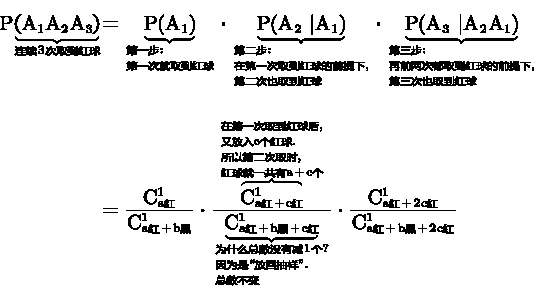
\includegraphics[width=0.85\textwidth]{/0094.pdf} \\
	
	上面可以看出: \\
	- 当 c红= 0 时, 就是正常的``放回抽样". \\
	- 当 c红= -1 时, 就是``不放回抽样". 即把之前步骤中取到的球, 拿走了, 不放回总体中. \\
	- 当 c红>0 时, 就是本例的``传染病模型".	



	
~\\
\hrule
~\\


	
	\section{全概率公式}
	
	全概率公式 Total Probability Theorem: \\	
	如果 $A_1, A_2, ..., A_n$ 构成一个``完备事件组", 即: (1) 这些事件两两互不相容,  (2)其``和"(或``并集")为全集 $\Omega$, (3) $P(A_i)>0$. \\
		
	则有:
$\boxed{
\sum_{\text{i}=1}^{\text{n}}{\ \left[ \text{P}\left( \text{A}_{\text{i}} \right) \cdot \text{P}\left( \text{B|A}_{\text{i}} \right) \right]}=\text{P}\left( \text{B} \right) 
}
$ \\

即有: $
\text{P}\left( \text{B} \right) =\underbrace{\text{P}\left( \text{A}_1 \right) \cdot \text{P}\left( \text{B|A}_1 \right) }+\underbrace{\text{P}\left( \text{A}_2 \right) \cdot \text{P}\left( \text{B|A}_2 \right) }+...+\underbrace{\text{P}\left( \text{A}_{\text{n}} \right) \cdot \text{P}\left( \text{B|A}_{\text{n}} \right) }
$ \\

	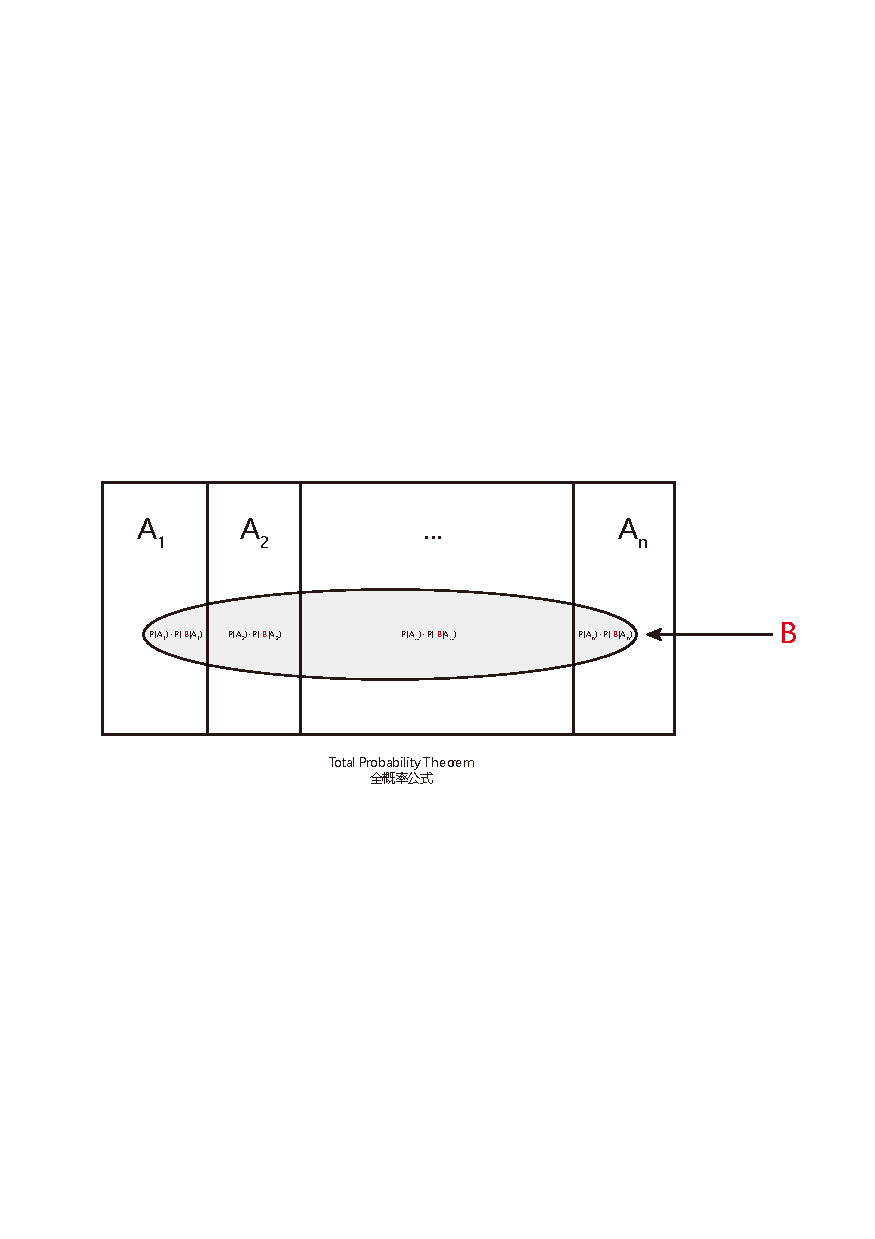
\includegraphics[width=1\textwidth]{/0095.pdf}
	
	
	\begin{myEnvSample}
		一个工厂, 有4条生产线, 情况如下: \\	
		\begin{tabular}{|l| l| l| l| l|}
			\hline
		 	&  生产线1  & 生产线2  &  生产线3 & 生产线4 \\
			\hline
			产量 &  15\% & 20\% & 30\% & 35\% \\
			\hline
			不合格率 &  0.05 & 0.04 & 0.03 & 0.02 \\
			\hline
		\end{tabular} \\
	
	问: 从该工厂的产品中, 任取一件, 是``不合格品"的概率? \\
	
	我们先设定事件: \\
	- $A_1$ : 表示是 生产线1 中的产品 \\
	- $A_2$ : 表示是 生产线2 中的产品 \\
	- $A_3$ : 表示是 生产线3 中的产品 \\
	- $A_4$ : 表示是 生产线4 中的产品 \\
	- $B$ : 表示是次品 \\
	
	那么, 你任取一件为不合格的概率, 不就是整个工厂总的不合格概率么?! 即 =P(B) \\		
		\begin{align*}
\text{P}\left( \text{B} \right) 
	&=\underset{\text{第1条生产线中(的条件下),\ 不合格品的概率}}{\underbrace{\overset{\text{产品属于生产线1的概率}}{\overbrace{\text{P}\left( \text{A}_1 \right) }}\cdot \overset{\text{生产线1中的次品率}}{\overbrace{\text{P}\left( \text{B|A}_1 \right) }}}}+\text{P}\left( \text{A}_2 \right) \cdot \text{P}\left( \text{B|A}_2 \right)  \\
	& +\text{P}\left( \text{A}_3 \right) \cdot \text{P}\left( \text{B|A}_3 \right) +\text{P}\left( \text{A}_4 \right) \cdot \text{P}\left( \text{B|A}_4 \right)\\
	&=\text{(15\%}\cdot 0.05\text{)}+\text{(20\%}\cdot 0.04\text{)}+\text{(30\%}\cdot 0.03\text{)}+\text{(35\%}\cdot 0.02\text{)}\\
	&=0.0315
		\end{align*}
	\end{myEnvSample}
	
	
	
\end{document}